\documentclass[preprint]{imsart}

\RequirePackage[OT1]{fontenc}
\RequirePackage{amsthm,amsmath}
\RequirePackage[numbers]{natbib}
\RequirePackage[colorlinks,citecolor=blue,urlcolor=blue]{hyperref}

\usepackage{amsfonts, amsopn, amssymb}
  \numberwithin{equation}{section}
\usepackage{color}
\usepackage{graphicx, subcaption, epstopdf}
\usepackage{hyperref}

\startlocaldefs
\numberwithin{equation}{section}
\theoremstyle{plain}
\newtheorem{theorem}{Theorem}[section]
\endlocaldefs

\newtheorem{assumption}[theorem]{Assumption}
\newtheorem{corollary}[theorem]{Corollary}
\newtheorem{definition}[theorem]{Definition}
\newtheorem{lemma}[theorem]{Lemma}
\newtheorem{proposition}[theorem]{Proposition}

\input{macros.tex}

% sets
\DeclareMathOperator{\cond}{cond}
\DeclareMathOperator{\col}{col}
\DeclareMathOperator{\row}{row}
\DeclareMathOperator{\area}{area}
\DeclareMathOperator{\base}{base}
\DeclareMathOperator{\height}{height}
\newcommand{\cR}{\mathcal{R}}

\begin{document}

\begin{frontmatter}
\title{CME 200 Workshop 4}
\runtitle{Workshop 4}
\begin{aug}
\runauthor{CME 200}
\author{October 18, 2013}
\end{aug}
\end{frontmatter}

\section{Questions and solutions}

\BNUM
\item Let $A$ be the matrix
$$
\BMAT 
1 & 2 & 0 & 2 & 1 \\
-1 & -2 & 1 & 1 & 0 \\
1 & 2 & -3 & -7 & -2
\EMAT
$$
Find (i) its rank, (ii) a basis for its row space, and (iii) a basis for its column space.

We row-reduce this matrix to obtain 
$$
\BMAT 
1 & 2 & 0 & 2 & 1 \\
0 & 0 & 1 & 3 & 1 \\
0 & 0 & 0 & 0 & 0
\EMAT.
$$
We deduce (i) $A$ has rank 2, (ii) the first two rows of $A$ form a basis for its row space
$$
\row(A) = \linspan\left(\left\{\BMAT 1 \\ 2 \\ 0 \\ 2 \\ 1 \EMAT,\BMAT -1 \\ -2 \\ 1 \\ 1 \\ 0 \EMAT\right\}\right),
$$
and (iii) the first and third columns of $A$ form a basis for its column space
$$
\cR(A) = \linspan\left(\left\{\BMAT 1 \\ -1 \\ 1 \EMAT,\BMAT 0 \\ 1 \\ -3 \EMAT\right\}\right).
$$
We know (ii) and (iii) because the first two rows of the reduced matrix are pivot rows and the first and third columns of the reduced matrix are pivot columns.

The first two rows of the row-reduced matrix also form a basis for the row space (of $A$). Row reduction takes linear combinations of the rows, so the row space is preserved by row reducing. The same cannot be said of the column space, so the first and third columns of the row-reduced matrix are NOT a basis for the columns space.

\item Find two matrices $A_1$ and $A_2$ such that (i) $\cond(A_1) \approx 10^6$ and $\det(A_1) = 1$ and (ii) $\cond(A_2) = 2$ and $\det(A_2) = 10^{-6}$.

Recall (from the first assignment) that the condition number is invariant under scalar multiplication, but the determinant is not. To find $A_1$ and $A_2$, we first find two matrices with the correct condition number, and then multiply these two matrices by a scalar to obtain the desired determinant. Two matrices with the correct condition numbers are
$$
\BMAT 10^6 & 0 \\ 0 & 1 \EMAT \text{ and }\BMAT 1 & 0 \\ 0 & 1 \EMAT.
$$
We multiply both matrices by $10^{-3}$ to obtain $A_1$ and $A_2$:
$$
A_1 = 10^{-3}\BMAT 10^6 & 0 \\ 0 & 1 \EMAT\text{ and }A_2 = 10^{-3}\BMAT 1 & 0 \\ 0 & 1 \EMAT. 
$$

\item Find an orthonormal basis for $\reals^2$ with Gram-Schmidt orthogonalization starting with the vectors
$$
a_1 = \BMAT 3 \\ -4 \EMAT,\,a_2 = \BMAT 1 \\ 1 \EMAT.
$$
The first vector in our orthonormal basis is simply $a_1$ normalized: 
$$
q_1 = \frac{a_1}{\norm{a_1}} = \BMAT \frac35 \\ -\frac45 \EMAT.
$$
To compute the second vector in our orthonormal basis, we first remove the component of $a_2$ along $q_1$: 
$$
w_2 = a_2 - (a_2^Tq_1)q_1 = \BMAT 1 \\ 1 \EMAT + \frac15\BMAT\frac35 \\ -\frac45 \EMAT = \BMAT \frac{28}{25} \\ \frac{21}{25} \EMAT.
$$
We then normalize $q_2$ to obtain the second vector in our orthonormal basis:
$$
q_2 = \frac{w_1}{\norm{w_2}} = \frac57\BMAT \frac{28}{25} \\ \frac{21}{25} \EMAT = \BMAT \frac{4}{5} \\ \frac{3}{5} \EMAT.
$$
\ENUM

\section{A geometric interpretation of the determinant}

Let $u\in\reals^2$ and $v\in\reals^2$ be the columns of a $2\times 2$ matrix $A$, \ie\
$$
A = \BMAT u & v \EMAT = \BMAT u_1 & v_1 \\ u_2 & v_2 \EMAT.
$$
$|\det(A)|$ is the area of the parallelogram whose vertices are the origin, $u$, $v$, and $u + v$ (see Figure \ref{fig:parallelogram}).

\begin{figure}
  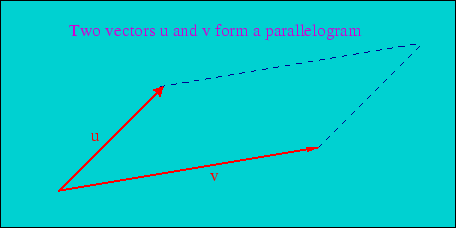
\includegraphics[scale=0.75]{parallelogram}
  \caption{The parallelogram formed by two vectors $u$ and $v$.}
  \label{fig:parallelogram}
\end{figure}

\begin{proof}
If we take the line segment between the origin and $u$ to be the base of the parallelogram, then the area of the parallelogram is
$$
\area = (\base)(\height) = (\norm{u})(\norm{v}\sin(\theta)),
$$
where $\theta$ is the angle between $u$ and $v$. We square both sides to obtain
\begin{align*}
\area^2 &= \norm{u}^2\norm{v}^2\sin^2(\theta) \\
&= \norm{u}^2\norm{v}^2(1 - \cos^2(\theta)) \\
&= \norm{u}^2\norm{v}^2\left(1 - \left(\frac{u^Tv}{\norm{u}\norm{v}}\right)^2\right) \\
&= \norm{u}^2\norm{v}^2 - (u^Tv)^2.
\end{align*}
We expand this expression in terms of the components of $u$ and $v$ to obtain
\begin{align*}
\area^2 &= (u_1^2 + u_2^2)(v_1^2 + v_2^2) - (u_1v_1 + u_2v_2)^2 \\
&= u_1^2v_2^2 + u_2^2v_1^2 - 2u_1v_1u_2v_2 \\
&= (u_1v_1 - u_2v_2)^2 \\
&= \det(A)^2.
\end{align*}
We take the square root of both sides to deduce $\area = |\det(A)|$.
\end{proof}

\end{document}
